\documentclass[../../../interview-questions.tex]{subfiles}

\begin{document}

\subsection{Redis数据类型}

Redis数据类型依赖于基础的数据结构,数据类型与数据结构的关系如图所示。

\begin{figure}[htbp]
	\centering
	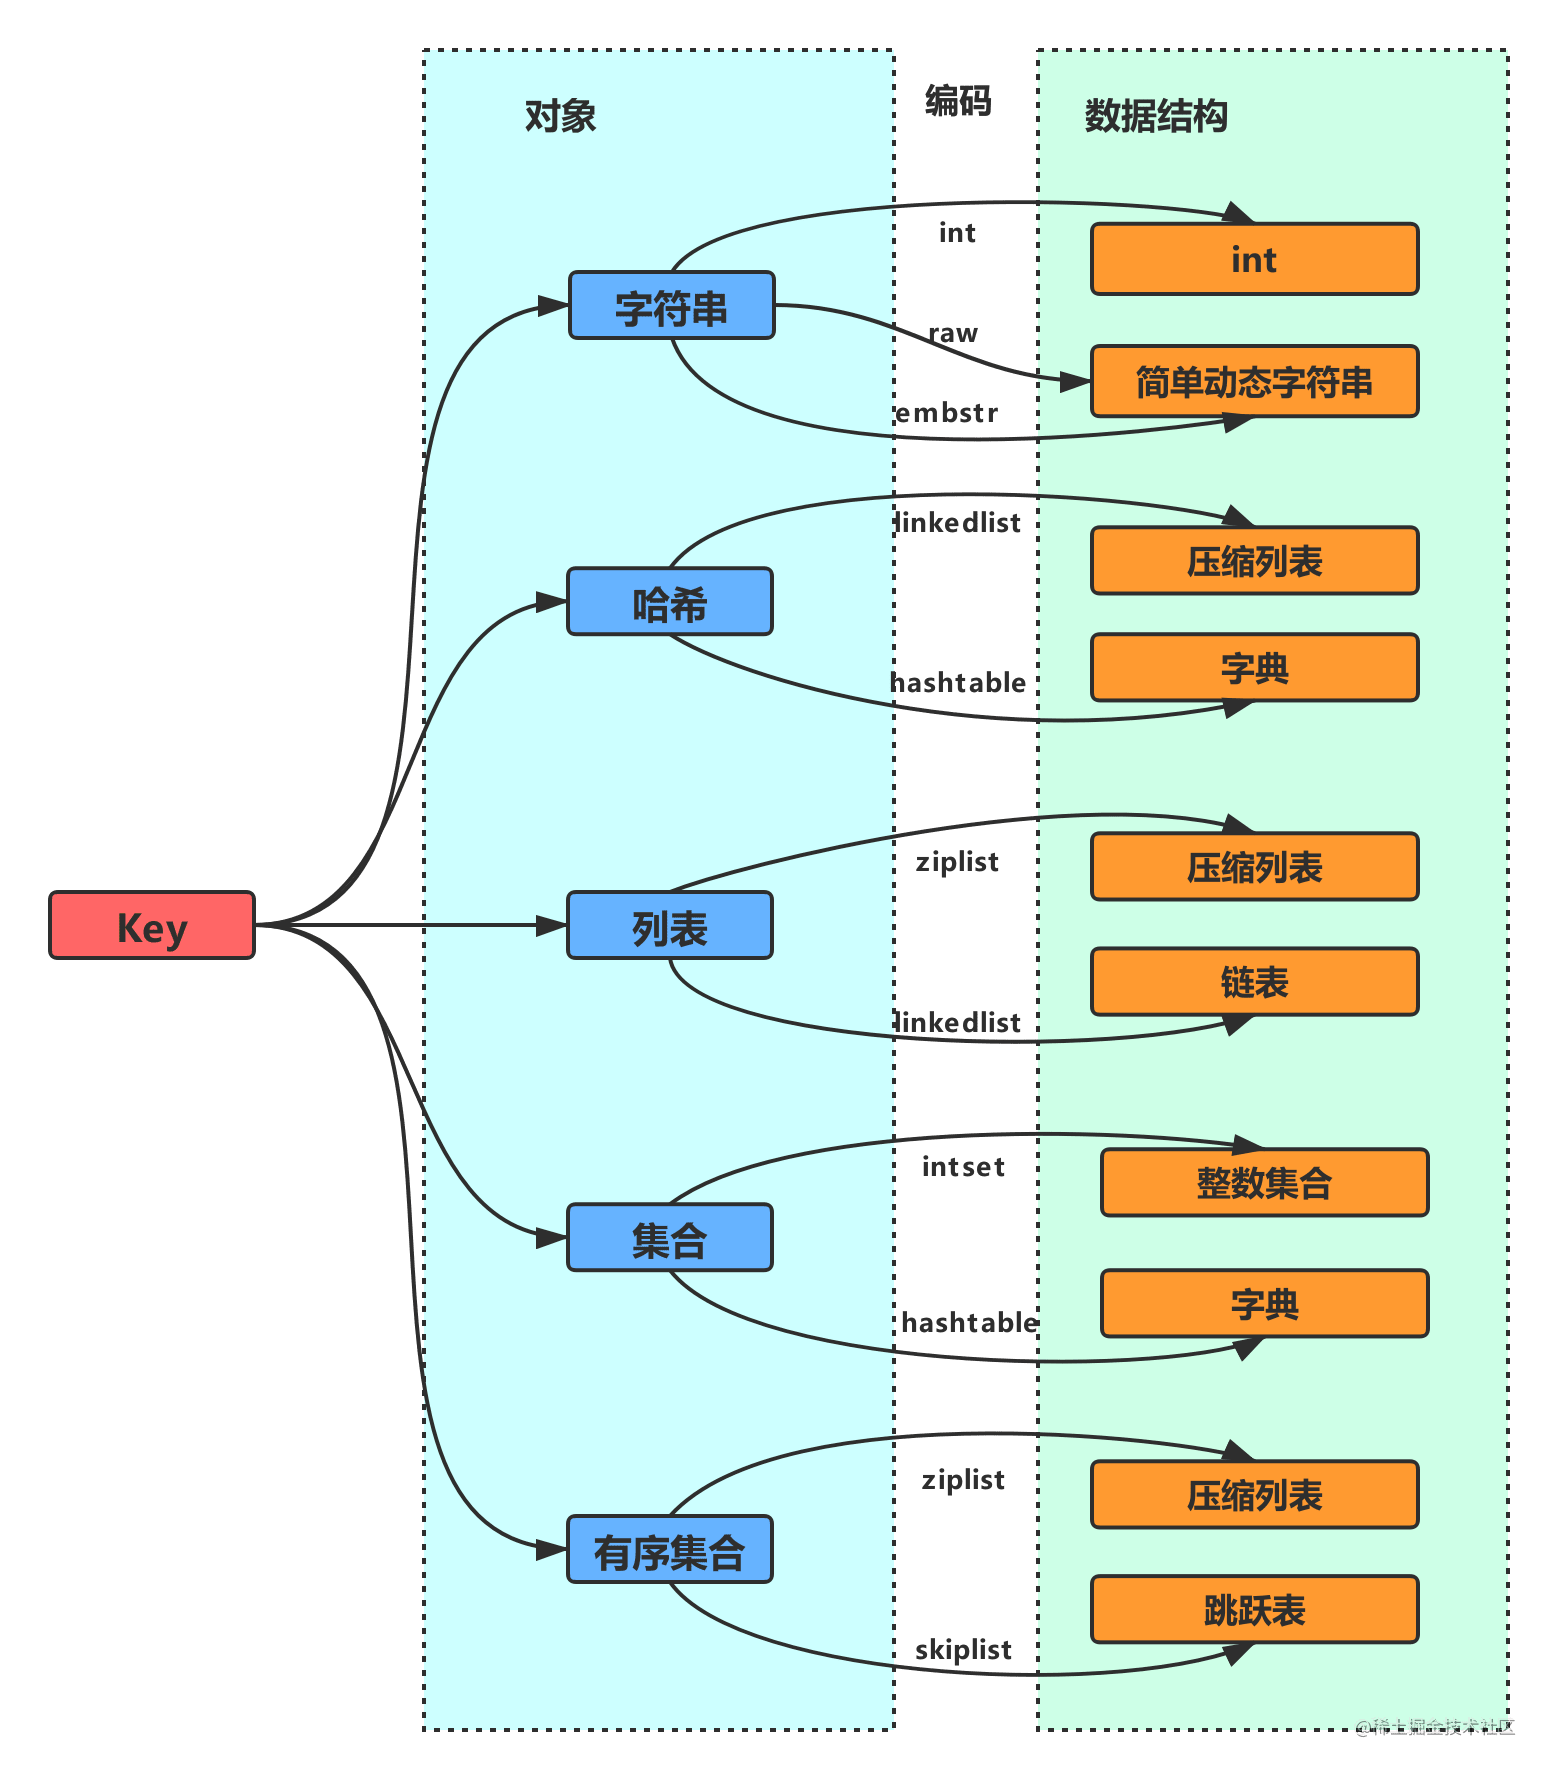
\includegraphics[scale=0.2]{redisdatatypepng.png}
	\caption{Redis数据类型与数据结构}
	\label{fig:redisdatatypepng}
\end{figure}

Redis支持数据类型\footnote{\url{https://redis.io/docs/data-types/}}。

\begin{enumerate}
    \item {Strings}
    \item {Lists}
    \item {Sets}
    \item {Hashes}
    \item {Sorted Sets}
    \item {Bitmaps}通常用来表示数据的状态,都是用来记录二进制位的操作,只有 0 和 1 两种状态。
    \item {HyperLogLogs}数据集中不重复的元素的个数,网页的访问量(UV):同一用户多次访问,也只能算作一个人。
    \item {Streams}
    \item {Geospatial indexes}
\end{enumerate}

\end{document}






